\chapter{Introduction} \label{intro}
\addcontentsline{toc}{chapter}{Introduction}

In recent years, robots and other technological aids have been spreading into more and more
areas of human endeavor. Nowadays, people encounter such machines in public spaces
like museums, airports, hospitals, and others\footnotei{.}{\url{https://spring-h2020.eu/about-spring/}}
Instead of just moving inside of a stationary
protective box in a manufacturing facility, public spaces place high demands on
the accuracy of localizing where the robot is, as the cost of a mistake can be high.

The problem of visual localization can be described as a task of finding
the position of a camera that took a query photo relative to a reference scene
representation\footnotei{.}{\url{https://www.visuallocalization.net}}
By the position in visual localization
6~parameters are meant (degrees of freedom---DoF), 3~of which are an absolute position in
reference coordinate system and the rest are the orientation of the camera.
A scene in general visual localization is a set
of RGB images, possibly associated with depth information per pixel (RGBD).
In the settings of this thesis, an \uv{explicit} scene representation
is used, unless otherwise said, meaning a 3D colored point cloud build from the \uv{implicit}
representation based wholly on images~\citep{SOTARendering}.

% https://europe.naverlabs.com/blog/methods-for-visual-localization/
As indicated, a solution to the problem is of great importance in autonomous robotics,
namely self-driving cars, terrestrial or aerial drones, and robots, also in augmented,
mixed or virtual reality applications. All of these examples interact through various
means with the surrounding environment suggesting that they are dependent upon location.\\

In our day-to-day lives, people typically meet so-called network-based positioning algorithms based on measuring
radio signals from various sources. These sources include Wi-Fi, Bluetooth Low Energy (BLE), Global Navigation
Satellite Systems (GNSS, such as GPS, Galileo), and cellular networks~\citep{Trogh2019}. All of these positioning
data sources suffer from shared limitations---they
can provide only 3~degrees of freedom position estimation, and the accuracy of such estimation can vary a lot.
Degradation outdoors comes from signal blockage or reflection due to high obstacles near the query position, 
solar storms, and indoors from signal damping through walls. Under the
best circumstances for a single query, GNSS can result in positioning within a few
centimeters\footnotei{,}{\url{https://www.gps.gov/systems/gps/performance/accuracy/}}
other methods can provide an estimate with uncertainty measured in even hundreds of meters. Network-based methods
find usage where an exact position is not that crucial, such as in asset tracking,
analyzing traffic patterns, transportation planning, security, surveillance, and population
movements tracking during disasters as a more specific example~\citep{Trogh2019}.

Network-based localization methods typically build upon the triangulation of a few measurements
of time-of-flight or signal strength from several sources, such as satellites, cell towers,
and access points, possibly combined with other techniques to reach better accuracy.
On the other hand, visual localization uses the rich visual information encoded in images to 
estimate the source camera's pose. One family of localization approaches that can be easily compared to
network-based methods relies on establishing an ideally high number of correspondences between
features of a query image and those of the scene representation. These correspondences are then
used to estimate the query image's camera pose with respect to the scene, typically more robustly
due to the large amount of them. Arguably, besides the different numbers of DoF these methods output,
visual localization may provide more reliable and accurate poses.

Thus, as the applications mentioned require higher accuracy, 6~DoF positions and fairly often
must work either directly indoors or at least reliably under various troublesome conditions for
network-based methods, visual localization has the potential to fulfill these
requirements accurately up to a few centimeters and
degrees\footnotei{.}{\url{https://www.visuallocalization.net/benchmark/}}

Visual localization brings its own challenges stemming mainly from the scene representation.
1) Illumination changes caused by artificial lighting and changes of the night and day
in the scene representation data, especially in query images, pose a significant problem
for both indoor and outdoor localization. The former type is a more challenging problem than the latter,
as indoors more complexities arise. 2) Furniture, equipment, and people add high dynamics
as they move significantly more than objects in urban settings. Also, previously unseen
objects may be added to the environment. All of these may cause
occlusions of possibly essential parts of the scene from the localization perspective. 3) Moreover, most
areas in buildings that stay the same (walls, floors) are largely textureless, which is problematic for many
feature-extracting approaches. Combined with dynamically moving objects that are, on the contrary,
more likely to be textured and thus resulting in better features to be worked with, feature
matches are often clustered in small unreliable areas leading to unstable pose estimates. 4) Even
in cases when features are more reliable, another issue arises as interiors are frequently
highly symmetric with repetitive elements on large (corridors, rooms,~\ldots) and small
(chairs, tables, doors,~\ldots) scales. 5) Finally, due to inherently smaller distances measured
in interiors compared to outdoors, a slight change in viewport leads to a substantial change in resulting
view~\citep{InLoc}.

Traditionally, camera position estimates can be computed during Structure-from-Motion (SfM)~\citep{SfM} or
(Visual) Simultaneous Localization and Mapping, (V)SLAM, see~\citet{SLAM}. The former is being used for creating
a 3D point cloud model of a given scene from reference photos alongside pose estimations of reference
cameras relative to the model built and nowadays may rather be used solely for 3D model creation, alongside
modern 3D scanners, such as LiDAR (an acronym for \uv{light detection and ranging}).
The latter is typically used by mobile robots moving within
a particular environment. When computed in real-time, the SfM and the VSLAM processes
are equivalent, sharing the same technical aspects and functionalities~\citep{VNAV}. Currently,
state-of-the-art approaches use matches between a 2D image and a 3D environment model, 
producing several candidate poses for a query image. Computed poses are verified and ranked based % TODO add citations
on sparse evidence, e.g., on the number
of inlier matches found by, e.g., RANSAC algorithm~\citep{RANSAC}. Due to the inherent candidate pose
instability and imperfections mentioned in the previous paragraph caused by the presence of repeated structures and
global ambiguities, a (weighted) inlier count has been shown as not a good
decision criterion~\citep{Burstiness}. Because of that,  InLoc paper authors~\citet{InLoc} proposed to compare
the query photo against a render of the scene from the candidate pose. The paper showed the pixel-wise comparison
to lead to a significantly better overall pose accuracy.

\begin{figure}
    \centering
    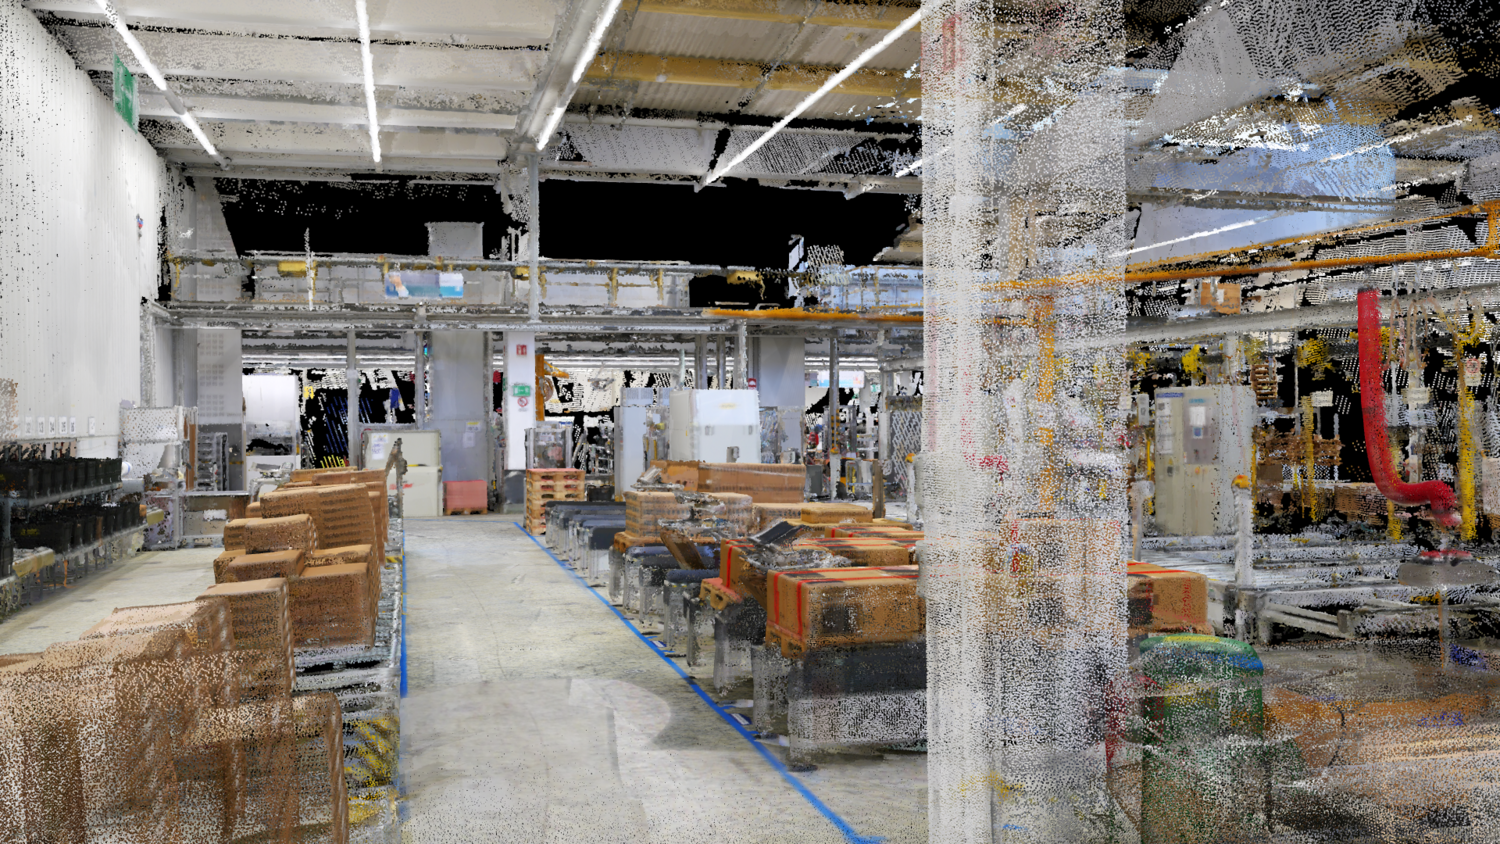
\includegraphics[width=.9\linewidth]{../graphics/0217_pyrender_artwin_render.png}
    \caption{A render of one of the datasets' point cloud. We can see an issue with using OpenGL's point
    primitive. Closer surfaces (the column, for instance) to the camera are not continuous but have holes
    and points that should be occluded by closer surfaces being visible. Fixed screen space point
    primitive is thus not a reliable way of rendering a point cloud without per-render pre-computations
    to set the correct pixel primitive.}\label{fig:pyrender_artwin_render}
\end{figure}

This thesis focuses on the verification step of the InLoc localization pipeline
as realistic rendering of point clouds\footnote{Point clouds are being used here
primarily because they are the direct output of SfM or triangulation of RGBD photo database and creation of
a mesh from such a point cloud is an unnecessary computational burden with an uncertain result when used
without human intervention.}
is a problem of its own. Arguably, the most widespread solution
for a point cloud rendering is the usage of the modern graphics APIs native primitive, such as \verb|GL_POINTS|
for OpenGL and WebGL. From a realistic rendering standpoint, this poses a problem because \uv{points are
rasterized as screen-aligned squares of a given window-space
size}\footnotei{.}{\url{https://www.khronos.org/opengl/wiki/Primitive}} Since this primitive has a fixed
size in the screen space, rendering of, for instance, a long hallway view results in nonuniform
\uv{surface} coverage. It does not matter whether the point cloud has a uniform spatial point
density produced by a LiDAR sensor or a nonuniform one produced by SfM. Walls farther from the camera may seem
like a solid surface, whereas closer ones can contain holes. The closer to the perspective camera, the bigger the
viewing angle of a point pair separated by a fixed-length line segment perpendicular to the viewing direction
is. With a specific distance-independent
screen space point dimension, it happens that the two point primitives visually split with no overlap
at a certain distance from the camera, see~\cref{fig:pyrender_artwin_render}. Transversely, such holes
may influence pixel-wise comparison in the pose verification step in InLoc as per-pixel computation of
descriptor distances between the render and the real query image would either be skipped because of missing
3D structure in the render or would result in the usage of a bad descriptor of a point that should not be visible
as it should be occluded by closer points (\uv{surfaces}) with, in general, different colors and neighborhoods.

The thesis explores three approaches to tackle the problem of realistic point cloud rendering. 1) Neural rendering
approach that uses a deep generative model to deal with occlusions, 2) a classical rendering approach
called ray marching paired with modeling points as spheres having the source point's color and radius equal
to the distance to the nearest neighbor to avoid holes in the resulting renders of flat surfaces, and 3)
surface splatting algorithm~\citep{SurfaceSplatting} that models points as oriented colored disks with radii determined the same
way as for ray marching-based renderer. Comparison to the work of~\citet{Bastien} is carried out on
the InLoc Dataset~\citep{InLoc} and all the renderers are also applied to a dataset from the ARTwin
project\footnotei{,}{\url{https://artwin-project.eu}} and the Phototourism
dataset\footnotei{.}{\url{https://www.cs.ubc.ca/research/image-matching-challenge/2021/data/}}
